% LaTeX resume using res.cls
\documentclass[line,margin,12pt]{res}
\usepackage{graphicx}
\usepackage{multicol}
%\usepackage{helvetica} % uses helvetica postscript font (download helvetica.sty)
%\usepackage{newcent}   % uses new century schoolbook postscript font
\begin{document}
\begin{multicols}{2}
\begin{flushright}
{\large \bf Valentin S. Petrov, PhD} \\
{\footnotesize
12, 30, Manufacturnaya str., Nizhny Novgorod, Russia, 603086 \\
tel. +7 xxx xxx xx xx \\
valentin.s.petrov@gmail.com\\
https://www.linkedin.com/in/vspetrov\\
https://github.com/vspetrov}
\end{flushright}

\columnbreak
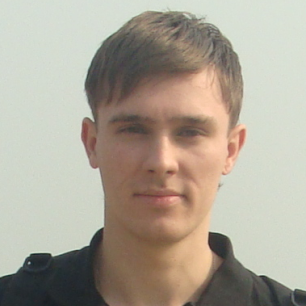
\includegraphics[scale=0.28]{image.png}
\end{multicols}


\begin{resume}

\section{FIELD OF INTEREST}
Nonlinear dynamics, synchronization theory, bifurcation theory, computer
modeling, parallel computing, Message Passing Interface, infiniband, collectives,
Computer Vision, algorithms, cardiomodeling

\section{EDUCATION} {}
\begin{itemize}
\item 10/2011 - 02/2012: Master Class program “Business English, Advanced”
\item 06/2011          : PhD Thesis defense in Physics-and-Mathematics
\item 06/2008 - 06/2011: PhD student in Nizhny Novgorod State University, Nizhny Novgorod Russia
\item 09/2003 - 06/2008: Student of the radio-physics faculty of Nizhny Novgorod State University
\item 09/2005 - 06/2008: student of the NNSU additional educational center, the English language course, specialization “Translator in the sphere of the professional communication” (Diploma $\#ППК 020487$)
\end{itemize}


\section{PROFESSIONAL EXPERIENCE} {}
\begin{itemize}
\item
{\sl 05/2014 - 09/2015: Senior Software Engineer at Intel}
\begin{itemize}
\item IntelMPI library (research, path-finding, development, optimization, benchmarking for high performance production MPI implementation)
\end{itemize}
\item
{\sl 03/2011 - 05/2014: Software Engineer at Itseez (http://itseez.com) }
\begin {itemize}
\item Software development for Mellanox (MPI Collective operations library FCA 3.0/HCOLL, OpenSHMEM, UPC/Gasnet)
\item ADAS - advanced driver assistance - real time traffic sign recognition with OpenCV
\end{itemize}
\item
{\sl 12/2004 - 12/2007: Intern Engineer at Joint Stock Company "Afrikantov Experimental Design Bureau for Mechanical Engineering"}
\begin{itemize}
\item FEM simulation and analysis with ANSYS
\end{itemize}
\end{itemize}


\section{ACADEMIC EXPERIENCE}{}
\begin{itemize}
\item 10/2010-11/2010: Visiting researcher, Golm University of Physics, Germany
\item 10/2009-11/2009: Visiting researcher, Leuven University, Belgium
\item 05/2009-06/2009: Visiting researcher, Golm University of Physics, Germany
\item 09/2008-12/2008: Visiting researcher, Leuven University, Belgium
\item 06/2007-07/2007: Visiting researcher, Leuven University, Belgium
\end{itemize}

\section{SKILLS}
{\sl Programming Languages}: C, C++, Python\\
{\sl Mathematical toolkits}: Matlab, Octave, ANSYS\\
{\sl Parallel programming}: MPI, Shmem, UPC/Gasnet, Nvidia CUDA, TBB, OpenMP, Intel Parallel Studio\\
{\sl Tools}: Mercurial/Git, Gdb, perf, gerrit, autotools, ClearQuest, Redmine\\
{\sl APIs}: verbs, psm, portals, rdmacm \\
{\sl English}: fluent \\
{\sl Others}: Latex \\

\section{AWARDS}
\begin{itemize}
\item Intel DPD Award, for valuable contribution into OpenFabric Interface, 2015
\item Winner of the scholarship of Academician GA Razuvaev, 2009-2010
\item Winner of the scholarship of Academician GA Razuvaev, 2010-2011
\item Winner of the Russian Federation President Scholarship, 2010-2011
\end{itemize}

\section{PUBLICATIONS}
\subsection{Papers}
\begin{enumerate}
\item V.N. Belykh, V.S. Petrov, G.V. Osipov, Dynamics of the Finite-dimensional Kuramoto Model: Global and Cluster Synchronization, Regul. Chaotic Dyn. (2015), 20 (1), pp. 37-48.
\item V. S. Petrov and G. V. Osipov. Interaction-based transition from passivity to excitability. Phys. Rev. E 90, 032916 (2014).
\item Di Lang, MS,Valentin Petrov, PhD, Qing Lou, PhD, Grigory Osipov,
PhD, Igor R. Efimov, PhD. Spatiotemporal control of heart rate in a
rabbit heart. Journal of Electrocardiology 44 (2011) 626 – 634.
\item V. S. Petrov, G. V. Osipov, and J. Kurths. Distant
synchronization through a passive medium, Physical Review E
(82) 026208, (2010).
\item V. S. Petrov, G. V. Osipov, and J. Kurths. Fibroblasts alter spiral
wave stability, Chaos (20) 045103 (2010).
\item A.K. Kryukov, V.S. Petrov, L.S. Averyanova, G.V. Osipov,
W.
Chen, O. Drugova and C.-K. Chan. Synchronization phenomena in
mixed media of passive, excitable and oscillatory cells. Chaos (13)
037129, 2008.
\item V.N. Belykh, G.V. Osipov, V.S. Petrov, J. Suykens, J.
Vandewalle. Cluster synchrsonization in oscillatory networks.
Chaos (13) 037106, 2008
\item V.S. Petrov, G.V. Osipov and J. A.K. Suykens. “Influence of
passive elements on the dynamics of oscillatory ensembles of
cardiac cells”. Phys. Rev. E (79) 046219, 2009
\item G. V. Osipov, O. I. Kanakov, C.-K. Chan, J. Kurths, S. K. Dana, L. S.
Averyanova, V. S. Petrov. “Synchronization Phenomena in
Networks of Oscillatory and Excitable Luo-Rudy Cells”. ''Complex
Dynamics in Physiological Systems: from heart to brain''.
Springer Science+Business Media B.V. 2009, p. 107-126.
\end{enumerate}
\subsection{Conference Proceedings}
\begin{enumerate}
\item V.S. Petrov, G.V. Osipov, O.I. Kanakov, C.K. Chan, J. Kurths. “Formation of synchronous clusters in networks of
cardiac cells”. // Proceedings of 3rd International IEEE
Scientific Conference on Physics and control (Physcon 2007),September 3rd-7th 2007 at the University of Potsdam, 2007, 1369
– 1373.
\item V.S. Petrov, G. V. Osipov, O. I. Kanakov, C.-K. Chan.
“Synchronous regimes in networks of cardiac cells”. // Book ofabstracts. International symposium on Synchronization in
complex networks, SynCoNet – 2007, July 2-4, Leuven, Belgium.
\item V.S. Petrov, G.V. Osipov, J. A.K. Suyukens. “Wave dynamics of oscillatory ensembles under the influence of
passive elements” // Proceedings of 17th International Workshop on Nonlinear Dynamics of Electronic Systems 2009,
Rapperswill, Switzerland, p. 82-85.
\item V.S. Petrov “Influence of passive elements on the
synchronization properties of oscillatory ensembles”,
Proceedings of the International Symposium on “Complex
Dynamical Systems and Applications”, Digha, India, December
4-6, 2009.
\item V.S. Petrov “Collective dynamics in mixed media of
oscillatory, excitable and passive cells”, international conference
Nonlinear Dynamics in Biological Systems, Taipei-Kenting, Taiwan, 2009
\end{enumerate}
\end{resume}

\end{document}
